\chapter{Mekanika Kuantum untuk Kimiawan: Sistem Model}\label{ch:b3:quantum-model-systems}

Tiga labu kecil berdiri di atas meja laboratorium, masing-masing berisi
larutan zat warna sianin dalam etanol: yang pertama magenta, yang kedua
biru, yang ketiga biru kehijauan pekat yang menyerap di daerah merah jauh.
Ketiga molekul itu tersusun serupa --- dua cincin bernitrogen yang identik
dihubungkan oleh rantai atom karbon --- dan hanya berbeda pada panjang rantai
itu, setiap kali dua atom karbon. Perpanjang rantainya, dan warnanya bergeser
ke arah merah. Seorang kimiawan pada tahun 1949 menjelaskan deret ini dengan
salah satu soal paling sederhana dalam mekanika kuantum: sebuah elektron yang
bebas bergerak di sepanjang garis yang panjangnya tetap, ``\omterm{def:b3:quantum-model-systems:box}{partikel dalam
kotak}''. Bab ini menyiapkan perangkat di balik penjelasan itu --- \omterm{def:b3:quantum-model-systems:operator}{operator},
\omterm{def:b3:quantum-model-systems:operator}{nilai eigen}, \omterm{thm:b3:quantum-model-systems:schrodinger}{persamaan Schrödinger} --- dan menyelesaikan sistem-sistem model
yang dipakai kimia setiap hari: kotak, \omterm{def:b3:quantum-model-systems:oscillator}{osilator harmonik} untuk ikatan yang
bervibrasi, \omterm{def:b3:quantum-model-systems:rotor}{rotor tegar} untuk molekul yang berputar, atom hidrogen, dan
penghalang yang dapat dilewati partikel ringan tanpa memiliki energi untuk
mendakinya.

\begin{recall}
Jilid Tahun 1 menunjukkan bahwa energi atom terkuantisasi (tingkat energi,
keadaan dasar dan keadaan tereksitasi, garis-garis spektrum hidrogen) dan
bahwa sebuah foton membawa $E = h\nu = hc/\lambda$. Jilid Tahun 2
menggambarkan elektron dengan fungsi gelombang $\psi$ yang kuadratnya
merupakan kepadatan peluang, memisahkan orbital hidrogen menjadi bagian
radial dan bagian sudut, serta menghitung simpulnya; jilid itu menerima
fungsi gelombang hidrogen begitu saja. Di sini fungsi-fungsi itu diturunkan,
di subbab 5. Dari fisika: momentum $p = mv$ dan panjang gelombang de Broglie
$\lambda = h/p$.
\end{recall}

\begin{omfigure}
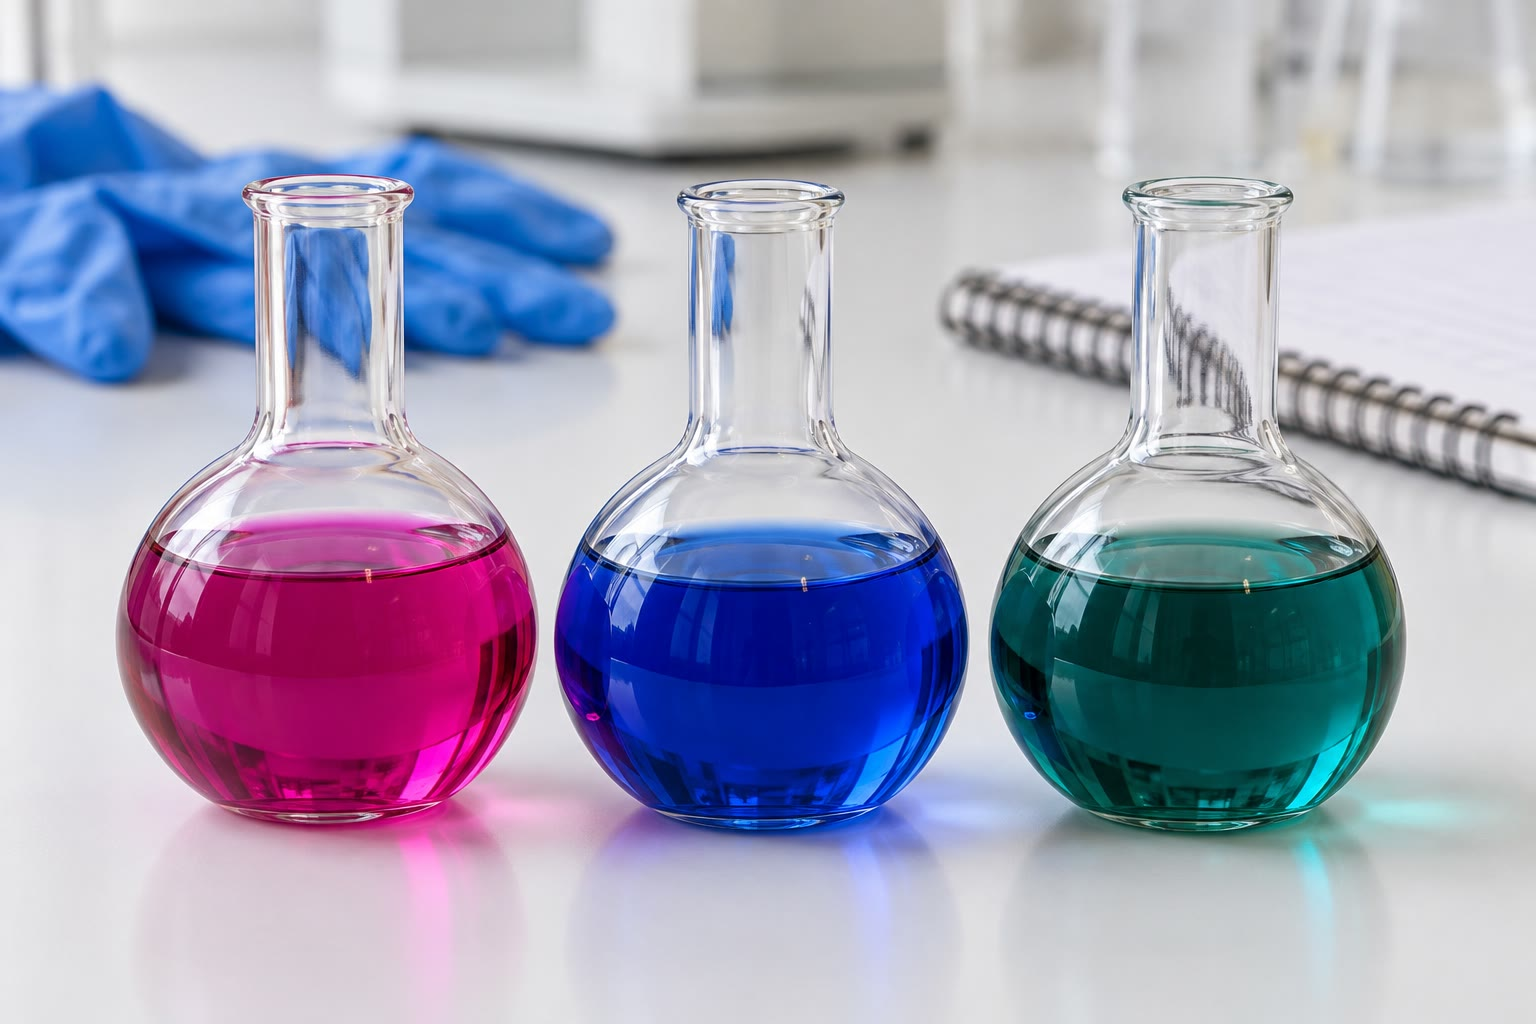
\includegraphics[width=0.62\linewidth]{images/book4/ai/b3-01-dyes.jpg}

{\small Larutan tiga zat warna sianin dari satu keluarga. Setiap pasangan
atom karbon yang ditambahkan pada rantai menggeser serapan ke arah merah.}
\end{omfigure}

\section{Operator, nilai eigen, dan persamaan Schrödinger}

Mekanika klasik memberi sebuah partikel posisi dan momentum pada setiap
saat. Mekanika kuantum memberinya sebuah keadaan, yaitu fungsi gelombang
$\psi$, dan mengganti setiap besaran terukur dengan suatu operasi yang
dikenakan pada $\psi$.

\begin{definition}[Operator, fungsi eigen, nilai eigen]\label{def:b3:quantum-model-systems:operator}
Yang disebut \emph{operator}\index{operator} $\hat A$ adalah aturan yang
mengubah suatu fungsi menjadi fungsi lain: $\hat A f = g$. Operator itu
linear jika $\hat A(\lambda f +
\mu g) = \lambda\hat Af + \mu\hat Ag$. Fungsi
tak nol $f$ yang memenuhi $\hat Af = a f$ untuk suatu bilangan $a$ disebut
\emph{fungsi eigen}\index{fungsi eigen} dari $\hat A$, dan $a$ adalah
\emph{nilai eigen}\index{nilai eigen} yang bersesuaian.
\end{definition}

\begin{example}[Dua operator: posisi dan momentum]\label{ex:b3:quantum-model-systems:xp}
Dalam satu dimensi, \omterm{def:b3:quantum-model-systems:operator}{operator} posisi mengalikan dengan $x$, $\hat x f = xf$,
dan \omterm{def:b3:quantum-model-systems:operator}{operator} momentum mendiferensialkan, $\hat p f = -\iu\hbar\,
\dd f/\dd x$, dengan $\hbar = h/2\pi$. Fungsi $\eu^{\iu kx}$ adalah \omterm{def:b3:quantum-model-systems:operator}{fungsi
eigen} dari $\hat p$ dengan \omterm{def:b3:quantum-model-systems:operator}{nilai eigen} $\hbar k$: gelombang dengan panjang
gelombang $\lambda = 2\pi/k$ mempunyai momentum $h/\lambda$, yaitu hubungan
de Broglie. Fungsi $\sin kx$ bukan \omterm{def:b3:quantum-model-systems:operator}{fungsi eigen} dari $\hat p$ (turunannya
berupa kosinus), tetapi merupakan \omterm{def:b3:quantum-model-systems:operator}{fungsi eigen} dari $\hat p^2 = -\hbar^2\,\dd^2/\dd x^2$, dengan \omterm{def:b3:quantum-model-systems:operator}{nilai eigen} $\hbar^2k^2$.
\end{example}

\begin{definition}[Operator Hermitian, nilai harapan]\label{def:b3:quantum-model-systems:hermitian}
Untuk dua fungsi yang lenyap di batas-batas daerahnya, kita tulis
$\langle f|g\rangle = \int f^*g\,\dd\tau$. Sebuah \omterm{def:b3:quantum-model-systems:operator}{operator} dikatakan
\emph{Hermitian}\index{operator Hermitian} jika $\langle f|\hat Ag\rangle = \langle \hat Af|g\rangle$ untuk semua $f$ dan $g$ semacam itu. Untuk keadaan
ternormalisasi $\psi$ ($\langle\psi|\psi\rangle = 1$), yang disebut
\emph{nilai harapan}\index{nilai harapan} dari $\hat A$ adalah
$\langle A\rangle = \langle\psi|\hat A\psi\rangle$: rata-rata dari banyak
pengukuran yang dilakukan pada sistem-sistem yang disiapkan secara identik.
\end{definition}

Aturan kerja kimia kuantum --- postulat-postulatnya --- kini dapat dinyatakan
sekaligus: setiap besaran terukur dinyatakan oleh sebuah \omterm{def:b3:quantum-model-systems:hermitian}{operator Hermitian};
sebuah pengukuran memberikan salah satu \omterm{def:b3:quantum-model-systems:operator}{nilai eigennya}; dan jika $\psi$
adalah \omterm{def:b3:quantum-model-systems:operator}{fungsi eigen} dari $\hat A$, setiap pengukuran pada keadaan itu
memberikan nilai yang sama, yaitu \omterm{def:b3:quantum-model-systems:operator}{nilai eigennya}.

\begin{theorem}[Operator Hermitian]\label{thm:b3:quantum-model-systems:hermitian-real}
\omterm{def:b3:quantum-model-systems:operator}{Nilai eigen} sebuah \omterm{def:b3:quantum-model-systems:hermitian}{operator Hermitian} adalah bilangan real. Dua \omterm{def:b3:quantum-model-systems:operator}{fungsi eigen}
dengan \omterm{def:b3:quantum-model-systems:operator}{nilai eigen} yang berbeda saling ortogonal: $\langle f_1|f_2\rangle = 0$.
\end{theorem}

\begin{proof}
Misalkan $\hat Af = af$. Maka $\langle f|\hat Af\rangle = a\langle f|f\rangle$
dan $\langle\hat Af|f\rangle = a^*\langle f|f\rangle$. \omterm{def:b3:quantum-model-systems:operator}{Operatornya} \omterm{def:b3:quantum-model-systems:hermitian}{Hermitian},
sehingga keduanya sama, dan $\langle f|f\rangle > 0$: $a = a^*$. Sekarang
misalkan $\hat Af_1
= a_1f_1$ dan $\hat Af_2 = a_2f_2$ dengan $a_1 \ne a_2$,
keduanya real. Maka $\langle f_1|\hat Af_2\rangle = a_2\langle f_1|f_2\rangle$
dan $\langle\hat Af_1|
f_2\rangle = a_1\langle f_1|f_2\rangle$; kesamaan
keduanya memberikan $(a_2 - a_1)
\langle f_1|f_2\rangle = 0$, sehingga
$\langle f_1|f_2\rangle = 0$.
\end{proof}

Hasil sebuah pengukuran adalah bilangan real; itulah sebabnya besaran
teramati harus \omterm{def:b3:quantum-model-systems:hermitian}{Hermitian}. Keortogonalan membuat orbital-orbital sebuah atom,
atau tingkat-tingkat sebuah kotak, menjadi himpunan keadaan bebas yang rapi.

\begin{definition}[Komutator]\label{def:b3:quantum-model-systems:commutator}
Yang disebut \emph{komutator}\index{komutator} dua \omterm{def:b3:quantum-model-systems:operator}{operator} adalah
$[\hat A,\hat B] =
\hat A\hat B - \hat B\hat A$. Kedua \omterm{def:b3:quantum-model-systems:operator}{operator} itu saling
komut jika komutatornya nol.
\end{definition}

\begin{example}[Komutator kanonik]\label{ex:b3:quantum-model-systems:canonical}
Untuk sembarang fungsi $f$, $\hat x\hat pf = -\iu\hbar xf'$ dan $\hat p\hat xf =
-\iu\hbar(f + xf')$. Selisihnya adalah $[\hat x,\hat p]f = \iu\hbar f$, sehingga
$[\hat x,\hat p] = \iu\hbar$: posisi dan momentum tidak saling komut. Hubungan
tunggal ini mendasari prinsip ketidakpastian dan, sebentar lagi, seluruh
spektrum \omterm{def:b3:quantum-model-systems:oscillator}{osilator harmonik}.
\end{example}

\begin{proposition}[Operator yang saling komut]\label{prop:b3:quantum-model-systems:commuting}
Jika $\hat A$ dan $\hat B$ saling komut dan $f$ adalah \omterm{def:b3:quantum-model-systems:operator}{fungsi eigen} dari
$\hat A$ dengan \omterm{def:b3:quantum-model-systems:operator}{nilai eigen} tak terdegenerasi $a$, maka $f$ juga \omterm{def:b3:quantum-model-systems:operator}{fungsi eigen}
dari $\hat B$.
\end{proposition}

\begin{proof}
$\hat A(\hat Bf) = \hat B\hat Af = a(\hat Bf)$: fungsi $\hat Bf$ adalah \omterm{def:b3:quantum-model-systems:operator}{fungsi
eigen} dari $\hat A$ dengan \omterm{def:b3:quantum-model-systems:operator}{nilai eigen} yang sama $a$, atau nol. Karena \omterm{def:b3:quantum-model-systems:operator}{nilai
eigen} itu tak terdegenerasi, $\hat Bf$ adalah kelipatan $f$, misalnya $bf$.
\end{proof}

\omterm{def:b3:quantum-model-systems:operator}{Operator} energi adalah Hamiltonian. Untuk partikel bermassa $m$ dalam
potensial $V$, energi klasik $p^2/2m + V$ menjadi sebuah \omterm{def:b3:quantum-model-systems:operator}{operator}.

\begin{definition}[Operator Hamiltonian]\label{def:b3:quantum-model-systems:schrodinger}
Yang disebut \emph{operator Hamiltonian}\index{operator Hamiltonian} untuk
partikel bermassa $m$ yang bergerak dalam potensial $V(\mathbf r)$ adalah
\[
\hat H = -\frac{\hbar^2}{2m}\nabla^2 + V(\mathbf r), \qquad \nabla^2 =
\frac{\partial^2}{\partial x^2} + \frac{\partial^2}{\partial y^2} +
\frac{\partial^2}{\partial z^2},
\]
dan untuk beberapa partikel, jumlah suku-suku kinetiknya dan semua energi
potensialnya.
\end{definition}

\begin{theorem}[Persamaan Schrödinger]\label{thm:b3:quantum-model-systems:schrodinger}
Keadaan-keadaan berenergi tertentu suatu sistem --- keadaan stasionernya ---
adalah \omterm{def:b3:quantum-model-systems:operator}{fungsi-fungsi eigen} dari Hamiltoniannya, dan energi-energi yang
diizinkan adalah \omterm{def:b3:quantum-model-systems:operator}{nilai-nilai eigennya}:
\[
\hat H\psi = E\psi,
\]
yaitu \emph{persamaan Schrödinger}\index{persamaan Schrödinger} yang tak
bergantung waktu. Fungsi $\psi$ yang dapat diterima bernilai tunggal, kontinu,
dan terintegralkan kuadrat (dapat dinormalisasi).
\end{theorem}
\begin{proof}[Kedudukan persamaan ini]
Ini adalah sebuah postulat, yang dibenarkan oleh akibat-akibatnya: tingkat
energi setiap sistem yang diselesaikan di bawah ini sesuai dengan spektroskopi.
Persamaan yang bergantung waktu, yang kasus stasionernya adalah persamaan ini,
termasuk ranah fisika.
\end{proof}

Syarat batas itulah yang menghasilkan kuantisasi: sebuah persamaan
diferensial mempunyai solusi untuk setiap $E$, tetapi hanya sekumpulan
diskret di antaranya yang tetap berhingga dan kontinu. Kimia lalu menjadi
soal memilih potensial, menyelesaikan persamaannya, dan membaca \omterm{def:b3:quantum-model-systems:operator}{nilai-nilai
eigennya}.

\begin{method}[Menyelesaikan model satu dimensi]\label{met:b3:quantum-model-systems:one-dimensional}
\begin{enumerate}
  \item Tuliskan potensial $V(x)$ dan Hamiltoniannya; bagilah ruang menjadi
        daerah-daerah tempat $V$ berbentuk sederhana.
  \item Selesaikan $-\frac{\hbar^2}{2m}\psi'' + V\psi = E\psi$ di setiap daerah:
        sinus dan kosinus jika $E > V$, eksponensial real jika $E < V$.
  \item Terapkan syarat-syaratnya: $\psi = 0$ di tempat $V$ tak berhingga;
        $\psi$ dan $\psi'$ kontinu pada undakan berhingga; $\psi \to 0$ di
        tak berhingga.
  \item Syarat-syarat itu hanya terpenuhi untuk $E$ tertentu: itulah
        tingkat-tingkat energinya.
  \item Normalisasikan setiap \omterm{def:b3:quantum-model-systems:operator}{fungsi eigen}; hitunglah simpulnya sebagai
        pemeriksaan (tingkat ke-$n$ suatu soal satu dimensi mempunyai
        $n - 1$ simpul).
\end{enumerate}
\end{method}

\section{Partikel dalam kotak}

\begin{definition}[Partikel dalam kotak, model elektron bebas]\label{def:b3:quantum-model-systems:box}
Sebuah \emph{partikel dalam kotak}\index{partikel dalam kotak} bergerak
bebas ($V = 0$) antara $x = 0$ dan $x = L$ dan tidak dapat keluar
($V = \infty$ di luarnya). Yang disebut \emph{model elektron
bebas}\index{model elektron bebas} untuk molekul terkonjugasi adalah model
yang memperlakukan elektron-elektron $\pi$-nya sebagai partikel-partikel
bebas dalam kotak yang panjangnya sama dengan panjang rantai terkonjugasi.
\end{definition}

\begin{theorem}[Tingkat energi kotak]\label{thm:b3:quantum-model-systems:box}
Tingkat-tingkat energi dan \omterm{def:b3:quantum-model-systems:operator}{fungsi-fungsi eigen} ternormalisasi untuk
partikel bermassa $m$ dalam kotak sepanjang $L$ adalah
\[
E_n = \frac{n^2h^2}{8mL^2}, \qquad \psi_n(x) = \sqrt{\frac2L}\,\sin\frac{n\pi
x}{L}, \qquad n = 1, 2, 3, \dots
\]
\end{theorem}

\begin{proof}
Di dalam kotak, $\psi'' = -k^2\psi$ dengan $k^2 = 2mE/\hbar^2$, sehingga
$\psi = A\sin kx +
B\cos kx$. Di luar, $\psi = 0$, dan kekontinuan memberikan
$\psi(0) = 0$, sehingga $B =
0$, serta $\psi(L) = 0$, sehingga $\sin kL = 0$
dengan $A \ne 0$: $kL = n\pi$, dengan $n$ bilangan bulat positif ($n = 0$
memberikan $\psi = 0$; $n$ negatif mengulang fungsi-fungsi yang sama). Maka
$E = \hbar^2k^2/2m = n^2\pi^2\hbar^2/2mL^2 = n^2h^2/8mL^2$. Akhirnya
$\int_0^L A^2\sin^2(n\pi x/L)\,\dd x = A^2L/2 = 1$ memberikan $A =
\sqrt{2/L}$.
\end{proof}

Tiga ciri berlaku untuk setiap sistem terikat: energi terendahnya tidak nol
(partikel itu tidak pernah dapat diam), tingkat-tingkat energinya makin
berjauhan ketika $n$ bertambah, dan makin rapat ketika kotaknya membesar
($E \propto 1/L^2$): kotak yang besar hampir bersifat klasik.

\begin{omfigure}
\begin{tikzpicture}
\begin{axis}[width=0.5\linewidth, height=6.4cm, xmin=-0.08, xmax=1.08,
  ymin=0, ymax=18.4, axis lines=left, xtick={0,1}, xticklabels={$0$,$L$},
  ytick={1,4,9,16}, yticklabels={$E_1$,$4E_1$,$9E_1$,$16E_1$},
  tick label style={font=\small}, xlabel={$x$}, title={\small $\psi_n$}]
\foreach \n in {1,4,9,16}{\addplot[gray!50, dashed, domain=0:1] {\n};}
\addplot[omDef, thick] table[x=x, y=p1] {figdata/out/bachelor-3-particle-in-box.dat};
\addplot[omDef, thick] table[x=x, y=p2] {figdata/out/bachelor-3-particle-in-box.dat};
\addplot[omDef, thick] table[x=x, y=p3] {figdata/out/bachelor-3-particle-in-box.dat};
\addplot[omDef, thick] table[x=x, y=p4] {figdata/out/bachelor-3-particle-in-box.dat};
\draw[very thick] (axis cs:0,0) -- (axis cs:0,18.4) (axis cs:1,0) -- (axis cs:1,18.4);
\end{axis}
\end{tikzpicture}\hspace{0.5em}%
\begin{tikzpicture}
\begin{axis}[width=0.5\linewidth, height=6.4cm, xmin=-0.08, xmax=1.08,
  ymin=0, ymax=18.4, axis lines=left, xtick={0,1}, xticklabels={$0$,$L$},
  ytick={1,4,9,16}, yticklabels={$n=1$,$n=2$,$n=3$,$n=4$},
  tick label style={font=\small}, xlabel={$x$}, title={\small $|\psi_n|^2$}]
\foreach \n in {1,4,9,16}{\addplot[gray!50, dashed, domain=0:1] {\n};}
\addplot[omThm, thick] table[x=x, y=d1] {figdata/out/bachelor-3-particle-in-box.dat};
\addplot[omThm, thick] table[x=x, y=d2] {figdata/out/bachelor-3-particle-in-box.dat};
\addplot[omThm, thick] table[x=x, y=d3] {figdata/out/bachelor-3-particle-in-box.dat};
\addplot[omThm, thick] table[x=x, y=d4] {figdata/out/bachelor-3-particle-in-box.dat};
\draw[very thick] (axis cs:0,0) -- (axis cs:0,18.4) (axis cs:1,0) -- (axis cs:1,18.4);
\end{axis}
\end{tikzpicture}

{\small Empat tingkat pertama \omterm{def:b3:quantum-model-systems:box}{partikel dalam kotak}, setiap fungsi digambar
pada tingkatnya sendiri (garis putus-putus). Kiri: $\psi_n$, dengan $n - 1$
simpul di dalam kotak. Kanan: kepadatan peluang $|\psi_n|^2$.}
\end{omfigure}

\begin{proposition}[Kotak kubus]\label{prop:b3:quantum-model-systems:box-3d}
Dalam kotak kubus bersisi $L$, $\psi = \psi_{n_x}(x)\psi_{n_y}(y)\psi_{n_z}(z)$
dan $E = (n_x^2 + n_y^2 + n_z^2)\,h^2/8mL^2$. Tripel-tripel berbeda dengan
jumlah kuadrat yang sama memberikan energi yang sama.
\end{proposition}

\begin{proof}
Dengan $V = 0$ di dalam kotak, $\hat H$ adalah jumlah tiga \omterm{def:b3:quantum-model-systems:operator}{operator} satu
dimensi, satu untuk setiap koordinat. Hasil kali tiga \omterm{def:b3:quantum-model-systems:operator}{fungsi eigen} satu
dimensi adalah \omterm{def:b3:quantum-model-systems:operator}{fungsi eigen} dari jumlah itu, dengan \omterm{def:b3:quantum-model-systems:operator}{nilai eigen} berupa
jumlah ketiga \omterm{def:b3:quantum-model-systems:operator}{nilai eigennya}; fungsi itu lenyap pada setiap sisi kubus,
sebagaimana disyaratkan.
\end{proof}

\begin{definition}[Tingkat terdegenerasi]\label{def:b3:quantum-model-systems:degenerate}
\omterm{def:b3:quantum-model-systems:operator}{Fungsi-fungsi eigen} yang bebas linear dengan \omterm{def:b3:quantum-model-systems:operator}{nilai eigen} yang sama disebut
\emph{tingkat terdegenerasi}\index{tingkat terdegenerasi}; banyaknya fungsi
itu adalah \emph{degenerasi}\index{degenerasi} $g$ dari energi tersebut.
\end{definition}

\begin{example}[Degenerasi dan simetri]\label{ex:b3:quantum-model-systems:cube}
Tingkat $n_x^2 + n_y^2 + n_z^2 = 6$ pada kubus berasal dari $(2,1,1)$,
$(1,2,1)$ dan $(1,1,2)$: $g = 3$. Regangkan kotak sedikit sepanjang $z$, maka
fungsi ketiga menjauh dari dua fungsi lainnya: \omterm{def:b3:quantum-model-systems:degenerate}{degenerasi} itu berasal dari
simetri kubus. Kaitan yang sama antara simetri dan \omterm{def:b3:quantum-model-systems:degenerate}{degenerasi} menata
\cref{ch:b3:point-groups,ch:b3:group-theory-applied}.
\end{example}

\subsection*{Zat warna terkonjugasi}

Dalam zat warna sianin yang simetris, rantai $j$ atom menghubungkan kedua
nitrogen (\(j = 5\), 7, 9 untuk ketiga zat warna dalam adegan pembuka), dan
elektron-elektron $\pi$-nya terdelokalisasi di sepanjang rantai itu. Rantai
$j$ atom membawa $N = j + 1$ elektron $\pi$: satu per karbon, ditambah
pasangan elektron bebas salah satu nitrogen yang terbagi ke seluruh kation.

\begin{proposition}[Panjang gelombang serapan menurut model elektron bebas]\label{prop:b3:quantum-model-systems:free-electron}
Jika $N$ elektron $\pi$ (bilangan genap) mengisi tingkat-tingkat kotak
sepanjang $L$, dua elektron per tingkat, maka serapan dengan panjang
gelombang terpanjang, dari tingkat terisi tertinggi $n = N/2$ ke tingkat
berikutnya, terletak pada
\[
\lambda = \frac{8mcL^2}{h(N+1)}.
\]
\end{proposition}

\begin{proof}
$\Delta E = E_{N/2+1} - E_{N/2} = [(N/2+1)^2 - (N/2)^2]\,h^2/8mL^2 =
(N+1)\,h^2/8mL^2$, dan $\lambda = hc/\Delta E$.
\end{proof}

\begin{example}[Kotak polos gagal, kotak yang diperpanjang berhasil]\label{ex:b3:quantum-model-systems:dyes}
% ledger: uvvis:cyanine, uvvis:carbocyanine, uvvis:dicarbocyanine, geo:C6H6.rCC
Ambil setiap ikatan dalam rantai sama dengan ikatan C--C benzena,
$l = \qty{139.7}{pm}$, sehingga rantai polos berukuran $(j - 1)l$. Untuk
ketiga zat warna ($N = 6$, 8, 10) rumus itu memberikan 147, 257 dan 374 nm,
jauh di bawah maksimum terukur, 524, 603 dan 711 nm dalam etanol.
Elektron-elektron itu tidak berhenti di atom nitrogen: mereka menyebar ke
dalam cincin. Perpanjang kotak sebesar $\delta$ di setiap ujung dan
cocokkan $\delta$ pada zat warna tengah: $\delta = \qty{222}{pm}$, kira-kira
satu setengah ikatan. Nilai $\delta$ yang sama lalu meramalkan 474 dan
732 nm untuk kedua zat warna lainnya, dengan selisih 10\,\% dan 3\,\%. Satu
panjang yang dapat disesuaikan menjelaskan sebuah keluarga warna (gambar di
bawah; angka-angkanya dihitung dalam skrip gambar itu).
\end{example}

\begin{omfigure}
\begin{tikzpicture}
\begin{axis}[width=0.5\linewidth, height=5.6cm, xmin=4, xmax=10,
  ymin=0, ymax=850, xtick={5,7,9}, axis lines=left,
  xlabel={atom dalam rantai, $j$}, ylabel={$\lambda_{\max}$ / nm},
  legend cell align=left, legend style={font=\small, at={(1.03,0.5)}, anchor=west, draw=none},
  tick label style={font=\small}, label style={font=\small}]
\addplot[only marks, mark=*, omThm] table[x=j, y=measured] {figdata/out/bachelor-3-particle-in-box-dyes.dat};
\addlegendentry{terukur (etanol)}
\addplot[omDef, thick, mark=square*] table[x=j, y=fitted] {figdata/out/bachelor-3-particle-in-box-dyes.dat};
\addlegendentry{kotak diperpanjang $\delta = 222$ pm}
\addplot[gray, dashed, mark=triangle*] table[x=j, y=bare] {figdata/out/bachelor-3-particle-in-box-dyes.dat};
\addlegendentry{rantai polos}
\end{axis}
\end{tikzpicture}

{\small Maksimum serapan ketiga zat warna sianin dibandingkan dengan \omterm{def:b3:quantum-model-systems:box}{model
elektron bebas}: rantai polos, dan kotak yang diperpanjang sebesar $\delta$
di setiap ujung, dengan $\delta$ dicocokkan pada zat warna tengah.}
\end{omfigure}

\begin{inthelab}[Mengukur sebuah deret zat warna]
Ketiga zat warna ditimbang (beberapa miligram), dilarutkan dalam etanol, lalu
diencerkan sampai absorbans pada maksimumnya berada antara 0.3 dan 1.
Spektrum masing-masing direkam antara 400 dan 800 nm dalam kuvet 1 cm
terhadap blangko etanol murni, dan $\lambda_{\max}$ dibaca di puncak pita
utama. Zat warna sianin berupa padatan yang menodai dan bersifat iritan:
sarung tangan dipakai, dan penimbangan dilakukan di lemari asam.
\end{inthelab}

\section{Osilator harmonik}

Di dekat dasar setiap sumur potensial yang mulus, $V \approx \frac12 k(x - x_e)^2$:
vibrasi kecil sebuah ikatan, sebuah atom dalam kristal, atau sebuah molekul
dalam sangkar, semuanya kira-kira harmonik.

\begin{definition}[Osilator harmonik, tetapan gaya, massa tereduksi, energi titik nol]\label{def:b3:quantum-model-systems:oscillator}
Yang disebut \emph{osilator harmonik}\index{osilator harmonik} adalah
partikel bermassa $m$ dalam potensial $V = \frac12 kx^2$; $k$ adalah
\emph{tetapan gaya}\index{tetapan gaya}, dan $\omega = \sqrt{k/m}$ frekuensi
sudut klasiknya. Molekul diatomik dengan massa atom $m_1$, $m_2$ bervibrasi
sebagai satu partikel dengan \emph{massa tereduksi}\index{massa tereduksi}
$\mu = m_1m_2/(m_1 + m_2)$ dalam potensial ikatannya. Energi tingkat terendah
sebuah osilator disebut \emph{energi titik nol}\index{energi titik nol}
osilator itu.
\end{definition}

\begin{definition}[Operator tangga]\label{def:b3:quantum-model-systems:ladder}
Dengan $x_0 = \sqrt{\hbar/m\omega}$, yang disebut \emph{operator
tangga}\index{operator tangga} adalah
\[
\hat a = \frac{1}{\sqrt2}\Big(\frac{\hat x}{x_0} + \frac{\iu x_0\hat p}{\hbar}\Big),
\qquad \hat a^\dagger = \frac{1}{\sqrt2}\Big(\frac{\hat x}{x_0} -
\frac{\iu x_0\hat p}{\hbar}\Big).
\]
\end{definition}

\begin{theorem}[Tingkat energi osilator harmonik]\label{thm:b3:quantum-model-systems:oscillator}
Tingkat-tingkat energi \omterm{def:b3:quantum-model-systems:oscillator}{osilator harmonik} adalah
\[
E_v = \big(v + \tfrac12\big)\hbar\omega = \big(v + \tfrac12\big)h\nu, \qquad v =
0, 1, 2, \dots,
\]
yang berjarak sama sebesar $h\nu$, dengan \omterm{def:b3:quantum-model-systems:oscillator}{energi titik nol} $\frac12h\nu$.
\end{theorem}

\begin{proof}
Dari $[\hat x,\hat p] = \iu\hbar$ diperoleh $[\hat a,\hat a^\dagger] = 1$ dan
$\hat H = \hbar\omega(\hat a^\dagger\hat a + \frac12)$. Tuliskan $\hat N =
\hat a^\dagger\hat a$. Maka $[\hat N,\hat a] = -\hat a$ dan $[\hat N,\hat
a^\dagger] = \hat a^\dagger$: jika $\hat N\psi = \nu\psi$, maka $\hat N(\hat
a\psi) = (\nu - 1)\hat a\psi$ dan $\hat N(\hat a^\dagger\psi) = (\nu + 1)\hat
a^\dagger\psi$; $\hat a$ menurunkan \omterm{def:b3:quantum-model-systems:operator}{nilai eigen} sebesar satu, dan
$\hat a^\dagger$ menaikkannya. Akan tetapi $\nu = \langle\psi|\hat a^\dagger\hat a\psi\rangle/\langle\psi|\psi
\rangle = \|\hat a\psi\|^2/\|\psi\|^2 \ge 0$: penurunan itu harus berhenti, dan
hal itu hanya terjadi pada fungsi dengan $\hat a\psi_0 = 0$, yang \omterm{def:b3:quantum-model-systems:operator}{nilai
eigennya} $\nu = 0$. Oleh karena itu, \omterm{def:b3:quantum-model-systems:operator}{nilai-nilai eigen} $\hat N$ adalah
$v = 0, 1, 2, \dots$, dan \omterm{def:b3:quantum-model-systems:operator}{nilai-nilai eigen} $\hat H$ adalah
$(v + \frac12)\hbar\omega$.
\end{proof}

\begin{proposition}[Fungsi-fungsi gelombang pertama]\label{prop:b3:quantum-model-systems:oscillator-functions}
Dalam koordinat tereduksi $y = x/x_0$,
\[
\psi_0 \propto \eu^{-y^2/2}, \quad \psi_1 \propto 2y\,\eu^{-y^2/2}, \quad
\psi_2 \propto (4y^2 - 2)\eu^{-y^2/2}, \quad \psi_3 \propto (8y^3 -
12y)\eu^{-y^2/2},
\]
yaitu polinomial Hermite dikalikan dengan fungsi Gauss. $\psi_v$ genap untuk
$v$ genap dan ganjil untuk $v$ ganjil.
\end{proposition}

\begin{proof}
$\hat a\psi_0 = 0$ berbunyi $y\psi_0 + \dd\psi_0/\dd y = 0$, yang solusinya
adalah fungsi Gauss. Setiap fungsi berikutnya diperoleh dengan mengenakan
$\hat a^\dagger$ pada fungsi sebelumnya, $\hat a^\dagger = \frac{1}{\sqrt2}(y - \dd/\dd y)$,
yang mengalikan polinomialnya dengan $2y$ lalu mengurangkan turunannya:
$1 \to 2y \to 4y^2 - 2 \to
8y^3 - 12y$ (sampai faktor pengali). Mengganti $y$
dengan $-y$ mengubah tanda $y$ dan tanda $\dd/\dd y$, sehingga
$\hat a^\dagger$ membalik paritas pada setiap langkah.
\end{proof}

\begin{omfigure}
\begin{tikzpicture}
\begin{axis}[width=0.66\linewidth, height=6.6cm, xmin=-4, xmax=4, ymin=0,
  ymax=4.6, axis lines=left, xlabel={$y = x/x_0$},
  ylabel={energi / $\hbar\omega$}, ytick={0.5,1.5,2.5,3.5},
  tick label style={font=\small}, label style={font=\small}]
\addplot[black, thick] table[x=y, y=V] {figdata/out/bachelor-3-harmonic-oscillator.dat};
\foreach \v in {0.5,1.5,2.5,3.5}{\addplot[gray!50, dashed, domain=-4:4] {\v};}
\addplot[omDef, thick] table[x=y, y=p0] {figdata/out/bachelor-3-harmonic-oscillator.dat};
\addplot[omDef, thick] table[x=y, y=p1] {figdata/out/bachelor-3-harmonic-oscillator.dat};
\addplot[omDef, thick] table[x=y, y=p2] {figdata/out/bachelor-3-harmonic-oscillator.dat};
\addplot[omDef, thick] table[x=y, y=p3] {figdata/out/bachelor-3-harmonic-oscillator.dat};
\addplot[only marks, mark=*, mark size=1.6pt, omThm] coordinates {(-1,0.5) (1,0.5)};
\node[omThm, font=\small, anchor=west] at (axis cs:2.0,0.2) {titik balik};
\draw[omThm, ->, thin] (axis cs:2.0,0.2) -- (axis cs:1.08,0.47);
\end{axis}
\end{tikzpicture}

{\small Potensial harmonik dengan empat tingkat energi dan fungsi gelombang
pertamanya, masing-masing digambar pada tingkatnya. Fungsi-fungsi gelombang
itu menjangkau melewati titik balik klasik ($y = \pm1$ untuk $v = 0$, titik
merah), tempat partikel klasik akan berhenti.}
\end{omfigure}

\begin{example}[Energi titik nol \ce{H2} dan \ce{D2}]\label{ex:b3:quantum-model-systems:zpe}
% ledger: diat:H2.we, diat:D2.we
Bilangan gelombang harmoniknya adalah $\tilde\omega_e = \qty{4401.2}{cm^{-1}}$
untuk \ce{H2} dan \qty{3115.5}{cm^{-1}} untuk \ce{D2}, dengan rasio $1.413$,
dekat dengan $\sqrt2$: ikatan dan \omterm{def:b3:quantum-model-systems:oscillator}{tetapan gayanya} sama, \omterm{def:b3:quantum-model-systems:oscillator}{massa tereduksinya}
dua kali lipat. \omterm{def:b3:quantum-model-systems:oscillator}{Energi titik nol} harmoniknya setengah dari nilai-nilai itu,
2200.6 dan \qty{1557.8}{cm^{-1}}, yaitu \qty{26.3}{kJ/mol} dan
\qty{18.6}{kJ/mol}. Sebuah molekul tidak pernah dapat kehilangan energi ini;
selisihnya antara isotop-isotop adalah sumber efek isotop dalam
\cref{ch:b3:statistical-thermo-applied,ch:b3:rate-theories}.
\end{example}

\section{Rotor tegar}

Molekul diatomik juga berputar terhadap pusat massanya. Jika diperlakukan
sebagai dua massa pada jarak tetap $r$, molekul itu adalah \omterm{def:b3:quantum-model-systems:rotor}{rotor tegar}
dengan momen inersia $I = \mu r^2$, yaitu \omterm{def:b3:quantum-model-systems:oscillator}{massa tereduksi} pada jarak $r$
dari sumbu.

\begin{definition}[Rotor tegar, harmonik bola]\label{def:b3:quantum-model-systems:rotor}
Yang disebut \emph{rotor tegar}\index{rotor tegar} adalah benda berbentuk
tetap yang berputar bebas; untuk molekul linear, $\hat H = \hat L^2/2I$, dengan
$\hat L^2$ \omterm{def:b3:quantum-model-systems:operator}{operator} kuadrat momentum sudut. \omterm{def:b3:quantum-model-systems:operator}{Fungsi-fungsi eigennya}, yang
hanya bergantung pada sudut $\theta$ dan $\phi$, adalah \emph{harmonik
bola}\index{harmonik bola} $Y_{l,m}(\theta,\phi)$, yang ditandai dengan $l =
0, 1, 2, \dots$ dan $m = -l, \dots, l$; untuk molekul, $l$ ditulis $J$.
\end{definition}

Rotor pada cincin (rotasi dalam sebuah bidang, terhadap sumbu tetap)
diselesaikan lebih dahulu; di situlah intinya.

\begin{theorem}[Cincin]\label{thm:b3:quantum-model-systems:ring}
Partikel bermomen inersia $I$ yang berputar dalam sebuah bidang mempunyai
tingkat energi $E_m = m^2\hbar^2/2I$ dengan $m = 0, \pm1, \pm2, \dots$; setiap
tingkat kecuali $m = 0$ terdegenerasi rangkap dua.
\end{theorem}

\begin{proof}
Satu-satunya koordinat adalah sudut $\phi$, dan $\hat H = -(\hbar^2/2I)\,
\dd^2/\dd\phi^2$. Solusi $\psi'' = -(2IE/\hbar^2)\psi$ adalah $\eu^{\iu
m\phi}$ dengan $m^2 = 2IE/\hbar^2$. Fungsi bernilai tunggal harus mempunyai
nilai yang sama di $\phi$ dan di $\phi + 2\pi$: $\eu^{2\pi\iu m} = 1$, sehingga
$m$ bilangan bulat. Fungsi dengan $m$ dan $-m$ mempunyai energi yang sama dan
saling bebas.
\end{proof}

\begin{theorem}[Tingkat energi rotor tegar]\label{thm:b3:quantum-model-systems:rotor}
$\hat L^2Y_{J,m} = J(J+1)\hbar^2\,Y_{J,m}$ dan $\hat L_zY_{J,m} = m\hbar\,
Y_{J,m}$, sehingga tingkat-tingkat energi \omterm{def:b3:quantum-model-systems:rotor}{rotor tegar} linear adalah
\[
E_J = \frac{\hbar^2}{2I}\,J(J+1), \qquad J = 0, 1, 2, \dots,
\]
masing-masing dengan \omterm{def:b3:quantum-model-systems:degenerate}{degenerasi} $g_J = 2J + 1$.
\end{theorem}
\admitted

Bukti umumnya, dengan \omterm{def:b3:quantum-model-systems:ladder}{operator tangga} untuk momentum sudut, dibahas dalam
kuliah yang lebih lanjut; berikut ini sebuah pemeriksaan. Dalam koordinat bola,
\[
\hat L^2 = -\hbar^2\Big[\frac{1}{\sin\theta}\frac{\partial}{\partial\theta}
\Big(\sin\theta\frac{\partial}{\partial\theta}\Big) +
\frac{1}{\sin^2\theta}\frac{\partial^2}{\partial\phi^2}\Big].
\]
Untuk $Y_{1,0} \propto \cos\theta$, kurung sikunya bernilai $\frac{1}{\sin\theta}(-2\sin\theta
\cos\theta) = -2\cos\theta$, sehingga $\hat L^2Y_{1,0} = 2\hbar^2Y_{1,0} = 1(1+1)\hbar^2
Y_{1,0}$. Untuk $Y_{1,\pm1} \propto \sin\theta\,\eu^{\pm\iu\phi}$ perhitungan
yang sama kembali memberikan $2\hbar^2$, dan $\hat L_z = -\iu\hbar\,\partial/\partial
\phi$ memberikan $\pm\hbar$.

\begin{proposition}[Harmonik bola real]\label{prop:b3:quantum-model-systems:real-harmonics}
Untuk $l = 1$, kombinasi $Y_{1,0}$, $(Y_{1,-1} - Y_{1,1})/\sqrt2$ dan
$\iu(Y_{1,-1} + Y_{1,1})/\sqrt2$ bernilai real dan sebanding dengan $z/r$,
$x/r$ dan $y/r$; untuk $l = 2$ konstruksi yang sama memberikan fungsi-fungsi
yang sebanding dengan $(3z^2 - r^2)$, $xz$, $yz$, $xy$ dan $x^2 - y^2$, dibagi
$r^2$.
\end{proposition}

\begin{proof}
$Y_{1,\pm1} \propto \mp\sin\theta\,\eu^{\pm\iu\phi}$ dengan konvensi tanda
yang lazim, sehingga selisih keduanya dibagi $\sqrt2$ bernilai
$\propto\sin\theta\cos\phi =
x/r$ dan jumlah berbobot $\iu$-nya
$\propto\sin\theta\sin\phi = y/r$; $\cos\theta = z/r$. Setiap kombinasi
\omterm{def:b3:quantum-model-systems:operator}{fungsi eigen} yang terdegenerasi tetap merupakan \omterm{def:b3:quantum-model-systems:operator}{fungsi eigen} dari $\hat L^2$
(dengan $l$ yang sama), meskipun bukan lagi \omterm{def:b3:quantum-model-systems:operator}{fungsi eigen} dari $\hat
L_z$. Kasus $l = 2$ memakai aljabar yang sama dengan $\sin^2\theta\,\eu^{\pm2\iu\phi}$
dan $\sin\theta\cos\theta\,\eu^{\pm\iu\phi}$.
\end{proof}

Inilah bagian sudut orbital $p$ dan $d$ yang digambar dalam jilid Tahun 2:
nama-namanya, $p_x$, $d_{xy}$, $d_{z^2}$, adalah bentuk Kartesius yang baru
saja diperoleh.

\begin{omfigure}
\begin{tikzpicture}[font=\small]
  \draw[->] (0,-0.2) -- (0,5.4) node[above] {$E/(\hbar^2/2I)$};
  \foreach \J/\E/\g in {0/0/1,1/2/3,2/6/5,3/12/7}{
    \pgfmathsetmacro{\y}{0.4*\E+0.1}
    \draw[omstate] (0.6,\y) -- (3.0,\y);
    \node[anchor=east] at (0.55,\y) {$\E$};
    \node[anchor=west] at (3.1,\y) {$J = \J$, \ $g = \g$};
  }
  \draw[<->, omThm] (2.4,0.9) -- (2.4,2.5) node[midway, left] {$4$};
  \draw[<->, omThm] (1.4,0.1) -- (1.4,0.9) node[midway, left] {$2$};
\end{tikzpicture}

{\small Tingkat-tingkat pertama \omterm{def:b3:quantum-model-systems:rotor}{rotor tegar} linear, $E_J = J(J+1)\,\hbar^2/2I$,
dengan \omterm{def:b3:quantum-model-systems:degenerate}{degenerasinya} $2J + 1$. Selisihnya tumbuh sebesar $2(J+1)$: itulah
penyebab garis-garis berjarak sama dalam \cref{ch:b3:rovibrational-spectroscopy}.}
\end{omfigure}

\begin{example}[Tingkat energi rotasi \ce{HCl}]\label{ex:b3:quantum-model-systems:hcl}
% ledger: diat:HCl.Be
Para spektroskopis menulis $E_J = hcB\,J(J+1)$ dengan tetapan rotasi $B =
\hbar/(4\pi cI)$ dalam bilangan gelombang. Untuk \ce{H^{35}Cl}, $B = \qty{10.593}{cm^{-1}}$:
tingkat-tingkat pertamanya terletak pada 0, 21.19, 63.56 dan
\qty{127.12}{cm^{-1}}, semuanya jauh di bawah energi termal pada suhu kamar,
$kT/hc = \qty{207}{cm^{-1}}$. Banyak tingkat rotasi terpopulasi; tingkat
vibrasi hanya satu ($\tilde\omega_e = \qty{2991}{cm^{-1}}$).
\end{example}

\section{Atom hidrogen dan penerowongan}

\subsection*{Atom hidrogen, diselesaikan}

Elektron bermuatan $-e$ di sekitar inti bermuatan $+e$ mempunyai $V = -e^2/
4\pi\varepsilon_0r$. Dengan \omterm{def:b3:quantum-model-systems:oscillator}{massa tereduksi} $\mu$ elektron dan proton,
\[
\hat H = -\frac{\hbar^2}{2\mu}\nabla^2 - \frac{e^2}{4\pi\varepsilon_0r},\qquad
\nabla^2 = \frac{1}{r^2}\frac{\partial}{\partial r}\Big(r^2\frac{\partial}{
\partial r}\Big) - \frac{\hat L^2}{\hbar^2r^2}.
\]
Bagian sudut $\nabla^2$ adalah \omterm{def:b3:quantum-model-systems:operator}{operator} rotor: solusinya terpisah menjadi
$\psi = R(r)\,Y_{l,m}(\theta,\phi)$, dan $R$ memenuhi persamaan radial
\[
-\frac{\hbar^2}{2\mu}\frac{1}{r^2}\frac{\dd}{\dd r}\Big(r^2\frac{\dd R}{\dd r}
\Big) + \Big[\frac{l(l+1)\hbar^2}{2\mu r^2} - \frac{e^2}{4\pi\varepsilon_0r}
\Big]R = ER.
\]
Rotasi menambahkan suku sentrifugal $l(l+1)\hbar^2/2\mu r^2$ yang menjauhkan
elektron dengan $l > 0$ dari inti.

\begin{theorem}[Tingkat energi atom hidrogen]\label{thm:b3:quantum-model-systems:hydrogen}
Tingkat-tingkat energi terikat atom mirip hidrogen dengan muatan inti $Ze$ adalah
\[
E_n = -\frac{\mu}{m_e}\,\frac{Z^2hcR_\infty}{n^2}, \qquad n = 1, 2, \dots,
\quad hcR_\infty = \frac{m_ee^4}{8\varepsilon_0^2h^2},
\]
dengan $l = 0, \dots, n - 1$; fungsi radial $1s$ dan $2p$ adalah $R_{10}
\propto \eu^{-Zr/a}$ dan $R_{21} \propto r\,\eu^{-Zr/2a}$, dengan $a =
(m_e/\mu)a_0$.
\end{theorem}

\begin{proof}[Bukti parsial]
Ambil $Z = 1$ dan cobalah $R = \eu^{-r/a}$ dengan $l = 0$. Maka $R' = -R/a$ dan
$\frac{1}{r^2}(r^2R')' = R/a^2 - 2R/(ar)$. Persamaan radialnya menjadi
$-\frac{\hbar^2}{2\mu}\big(\frac{1}{a^2} - \frac{2}{ar}\big) - \frac{e^2}{4\pi
\varepsilon_0r} = E$ untuk semua $r$: suku-suku dalam $1/r$ saling meniadakan
jika $a =
4\pi\varepsilon_0\hbar^2/\mu e^2$, dan kemudian $E = -\hbar^2/2\mu a^2 = -\mu
e^4/8\varepsilon_0^2h^2$, yaitu tingkat $n = 1$. Dengan $R = r\eu^{-r/b}$ dan
$l = 1$, substitusi yang sama menyisakan suku-suku dalam $1/r^2$ (yang
meniadakan suku sentrifugal), dalam $1/r$ (yang saling meniadakan jika
$b = 2a$) dan sebuah tetapan, $E =
-\hbar^2/2\mu b^2$, seperempat dari nilai
sebelumnya: tingkat $n = 2$. Kasus umumnya, sebuah polinomial dikalikan
$\eu^{-r/na}$ yang deretnya harus berhenti agar tetap dapat dinormalisasi,
dibahas dalam kuliah yang lebih lanjut.
\end{proof}

\begin{omfigure}
\begin{tikzpicture}
\begin{axis}[width=0.66\linewidth, height=5.4cm, xmin=0, xmax=12,
  ymin=-0.15, ymax=1.05, axis lines=left, samples=160, domain=0:12,
  xlabel={$r/a$}, ylabel={$R(r)$, diskalakan},
  legend cell align=left, legend style={font=\small, draw=none}, tick label style={font=\small},
  label style={font=\small}]
\addplot[omDef, thick] {exp(-x)}; \addlegendentry{$R_{10} \propto \eu^{-r/a}$}
\addplot[omThm, thick] {(1-x/2)*exp(-x/2)}; \addlegendentry{$R_{20} \propto (1 - r/2a)\eu^{-r/2a}$}
\addplot[omProp, thick] {0.5*x*exp(-x/2)/exp(-1)}; \addlegendentry{$R_{21} \propto r\,\eu^{-r/2a}$}
\addplot[gray, dashed] {0};
\end{axis}
\end{tikzpicture}

{\small Fungsi radial atom hidrogen, dari solusi-solusi di atas (masing-masing
diskalakan agar maksimumnya mendekati 1). $R_{20}$ mempunyai satu simpul
radial di $r = 2a$; $R_{21}$ lenyap di inti, terdorong keluar oleh suku
sentrifugal.}
\end{omfigure}

\begin{example}[Energi ionisasi hidrogen]\label{ex:b3:quantum-model-systems:ie}
% ledger: const:RyhcEV, const:me, const:mp
$hcR_\infty = \qty{13.6057}{eV}$ dan $\mu/m_e = 1/(1 + m_e/m_p) = 0.999456$,
sehingga $-E_1 = \qty{13.598}{eV}$: energi ionisasi hidrogen terukur, sampai
digit terakhir yang diberikan dalam jilid Tahun 1. \omterm{def:b3:quantum-model-systems:oscillator}{Massa tereduksi} mengubah
angka penting keempat.
\end{example}

\subsection*{Penerowongan}

\begin{definition}[Penerowongan, peluang transmisi]\label{def:b3:quantum-model-systems:tunnelling}
Yang disebut \emph{penerowongan}\index{penerowongan} adalah lewatnya sebuah
partikel melalui daerah tempat energinya lebih rendah daripada energi
potensial, sesuatu yang terlarang dalam mekanika klasik. Yang disebut
\emph{peluang transmisi}\index{peluang transmisi} $T$ sebuah penghalang
adalah fraksi partikel datang yang ditemukan di seberangnya.
\end{definition}

\begin{proposition}[Penghalang tipis dan tebal]\label{prop:b3:quantum-model-systems:barrier}
Di dalam penghalang setinggi $V_0 > E$, $\psi$ merupakan kombinasi
$\eu^{\pm\kappa x}$ dengan $\kappa = \sqrt{2m(V_0 - E)}/\hbar$. Untuk
penghalang persegi selebar $a$,
\[
T = \Big[1 + \frac{\sinh^2(\kappa a)}{4\varepsilon(1-\varepsilon)}\Big]^{-1},
\qquad \varepsilon = \frac{E}{V_0},
\]
dan untuk penghalang tebal ($\kappa a \gg 1$), $T \approx 16\varepsilon(1-\varepsilon)
\,\eu^{-2\kappa a}$.
\end{proposition}

\begin{proof}[Bukti parsial]
Di dalam penghalang, \omterm{thm:b3:quantum-model-systems:schrodinger}{persamaan Schrödinger} berbunyi $\psi'' = \kappa^2\psi$,
yang solusinya adalah kedua eksponensial itu. Menyambungkan $\psi$ dan
$\psi'$ di kedua dinding dengan gelombang $\eu^{\pm\iu kx}$ di luar
menghasilkan empat persamaan linear; solusinya, satu halaman aljabar, adalah
rumus untuk $T$, yang diterima tanpa bukti. Untuk $\kappa a$ yang besar,
$\sinh\kappa a \approx \frac12\eu^{\kappa a}$ mendominasi dan memberikan bentuk
penghalang tebal.
\end{proof}

Faktor penentunya adalah $\eu^{-2\kappa a}$, dan $\kappa \propto \sqrt m$:
\omterm{def:b3:quantum-model-systems:tunnelling}{penerowongan} adalah urusan partikel-partikel paling ringan, pertama-tama
elektron, kemudian proton, dan jauh lebih sedikit deuteron.

\begin{omfigure}
\begin{tikzpicture}
\begin{axis}[width=0.66\linewidth, height=5.6cm, xmin=0, xmax=1, ymode=log,
  ymin=1e-10, ymax=1e-1, axis lines=left, xlabel={$E/V_0$},
  ylabel={peluang transmisi $T$},
  legend cell align=left, legend style={font=\small, at={(0.03,0.97)}, anchor=north west, draw=none},
  tick label style={font=\small}, label style={font=\small}]
\addplot[omDef, thick] table[x=eps, y=TH] {figdata/out/bachelor-3-tunnelling.dat};
\addlegendentry{proton}
\addplot[omThm, thick, dashed] table[x=eps, y=TD] {figdata/out/bachelor-3-tunnelling.dat};
\addlegendentry{deuteron}
\end{axis}
\end{tikzpicture}

{\small \omterm{def:b3:quantum-model-systems:tunnelling}{Peluang transmisi} melalui penghalang model setinggi 0.40 eV dan
selebar 50 pm. Pada setengah tinggi penghalang, proton lolos kira-kira 58
kali lebih sering daripada deuteron (skala logaritmik).}
\end{omfigure}

\begin{remark}[Di mana penerowongan tampak]\label{rem:b3:quantum-model-systems:where}
Molekul amonia mengalami inversi, atom nitrogennya menembus bidang ketiga
hidrogen, dengan menerowong melalui penghalang yang rendah; transfer proton dan atom hidrogen dalam enzim menunjukkan efek
isotop kinetik yang jauh lebih besar daripada yang diramalkan
\cref{ch:b3:rate-theories} tanpa \omterm{def:b3:quantum-model-systems:tunnelling}{penerowongan}; dan mikroskop \omterm{def:b3:quantum-model-systems:tunnelling}{penerowongan}
payar mencitrakan atom-atom tunggal pada permukaan melalui arus elektron yang
menerowong melintasi celah vakum yang lebarnya beberapa persepuluh nanometer,
arus yang turun sepuluh kali lipat untuk setiap tambahan 0.1 nm.
\end{remark}

\begin{history}[Schrödinger, 1926]
\begin{minipage}[t]{0.72\linewidth}
Dalam empat makalah yang ditulis pada paruh pertama tahun 1926, Erwin
Schrödinger mengganti aturan-aturan kuantum atom Bohr dengan sebuah
persamaan gelombang, menyelesaikannya untuk atom hidrogen, osilator, dan
rotor, serta memperoleh kembali tingkat-tingkat energi yang telah diukur
oleh spektroskopi. Bilangan-bilangan bulat yang dipaksakan Bohr secara manual
kini muncul dengan sendirinya, sewajar banyaknya simpul pada dawai yang
bergetar. Ia berbagi Hadiah Nobel Fisika 1933 dengan Paul Dirac.
\end{minipage}\hfill
\begin{minipage}[t]{0.22\linewidth}\vspace{0pt}
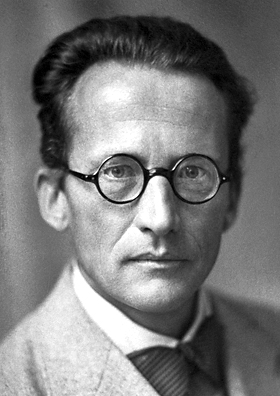
\includegraphics[width=\linewidth]{images/book4/schrodinger-1933.jpg}\par
{\footnotesize Schrödinger pada tahun 1933.}
\end{minipage}
\end{history}

\section{Latihan}

\begin{exercise}[$\star$]\label{exo:b3:quantum-model-systems:1}
Sebuah elektron terkurung dalam kotak sepanjang (a) \qty{1.00}{nm}, (b)
\qty{0.50}{nm}. Hitunglah $E_1$ dalam joule dan elektronvolt, serta panjang
gelombang transisi $n = 1 \to 2$.
\end{exercise}

\begin{exercise}[$\star$]\label{exo:b3:quantum-model-systems:2}
Daftarlah lima tingkat terendah \omterm{def:b3:quantum-model-systems:box}{partikel dalam kotak} kubus, dalam satuan
$h^2/8mL^2$, beserta \omterm{def:b3:quantum-model-systems:degenerate}{degenerasinya}.
\end{exercise}

\begin{exercise}[$\star$]\label{exo:b3:quantum-model-systems:3}
Hitunglah \omterm{def:b3:quantum-model-systems:commutator}{komutator} $[\hat x^2,\hat p]$ dan $[\hat p^2,\hat x]$ dengan
mengenakannya pada sebuah fungsi $f(x)$.
\end{exercise}

\begin{exercise}[$\star$]\label{exo:b3:quantum-model-systems:4}
% ledger: diat:HCl.Be
Dengan $B = \qty{10.593}{cm^{-1}}$ untuk \ce{H^{35}Cl}, berikan energi (dalam
\unit{cm^{-1}}) dan \omterm{def:b3:quantum-model-systems:degenerate}{degenerasi} tingkat $J = 0$ sampai 3, serta momen inersia
molekul itu.
\end{exercise}

\begin{exercise}[$\star\star$]\label{exo:b3:quantum-model-systems:5}
Untuk keadaan $\psi_n$ \omterm{def:b3:quantum-model-systems:box}{partikel dalam kotak}, hitunglah $\langle x\rangle$ dan
$\langle x^2\rangle$. Hitunglah $\langle x^2\rangle$ untuk $n = 1$ dan
bandingkan dengan nilai klasik $L^2/3$ untuk partikel yang berpeluang sama
untuk berada di mana saja.
\end{exercise}

\begin{exercise}[$\star\star$]\label{exo:b3:quantum-model-systems:6}
% ledger: diat:H2.we, diat:D2.we
Hitunglah \omterm{def:b3:quantum-model-systems:oscillator}{energi titik nol} harmonik \ce{H2} dan \ce{D2} dalam
\unit{kJ/mol} dari $\tilde\omega_e = \qty{4401.2}{cm^{-1}}$ dan
\qty{3115.5}{cm^{-1}}, serta selisihnya. Rasio bilangan gelombang berapakah
yang diharapkan dari \omterm{def:b3:quantum-model-systems:oscillator}{massa tereduksinya}, dan seberapa dekat rasio terukurnya?
\end{exercise}

\begin{exercise}[$\star\star$]\label{exo:b3:quantum-model-systems:7}
Fungsi $\phi = Nx(L - x)$ adalah tebakan kasar untuk keadaan dasar kotak.
Normalisasikan fungsi itu, lalu hitunglah tumpang-tindihnya
$\langle\psi_1|\phi\rangle$ dengan keadaan dasar yang sebenarnya.
\end{exercise}

\begin{exercise}[$\star\star$]\label{exo:b3:quantum-model-systems:8}
Tunjukkan bahwa $\hat p = -\iu\hbar\,\dd/\dd x$ \omterm{def:b3:quantum-model-systems:hermitian}{Hermitian} untuk fungsi-fungsi
yang lenyap di kedua ujung suatu selang, dan bahwa $\hat x\hat p$ tidak.
\end{exercise}

\begin{exercise}[$\star\star$]\label{exo:b3:quantum-model-systems:9}
Modelkan heksa-1,3,5-triena sebagai enam elektron $\pi$ dalam kotak sepanjang
$6l$, $l =
\qty{139.7}{pm}$ (lima ikatan ditambah setengah ikatan di setiap
ujung). Ramalkan panjang gelombang serapan pertamanya. Apakah molekul itu
berwarna?
\end{exercise}

\begin{exercise}[$\star\star\star$]\label{exo:b3:quantum-model-systems:10}
Untuk penghalang model pada gambar ($V_0 = \qty{0.40}{eV}$, $a = \qty{50}{pm}$)
pada $E = V_0/2$, hitunglah $\kappa$ untuk proton dan untuk deuteron serta,
dengan rumus penghalang tebal, rasio $T_H/T_D$. Bandingkan dengan rasio
eksaknya, 58.
\end{exercise}

\begin{exercise}[$\star\star\star$]\label{exo:b3:quantum-model-systems:11}
Perlakukan keenam elektron $\pi$ benzena sebagai partikel pada cincin
berjari-jari \qty{139.7}{pm} (jarak C--C sama dengan jari-jari heksagon
beraturan). Isilah tingkat-tingkatnya, lalu hitunglah panjang gelombang
transisi dari tingkat terisi tertinggi ke tingkat kosong terendah.
\end{exercise}

\begin{exercise}[$\star\star\star$]\label{exo:b3:quantum-model-systems:12}
Untuk keadaan $1s$ hidrogen, $\psi = (\pi a^3)^{-1/2}\eu^{-r/a}$. Hitunglah
\omterm{def:b3:quantum-model-systems:hermitian}{nilai harapan} $\langle r\rangle$ dan $\langle V\rangle$, dan periksalah bahwa
$\langle V\rangle = 2E_1$. (Gunakan $\int_0^\infty r^n\eu^{-\beta r}\dd r =
n!/\beta^{n+1}$.)
\end{exercise}

\section{Soal: Berapa Panjang Sebuah Zat Warna?}

\begin{problem}[{Soal akhir pekan --- model elektron bebas untuk tiga zat
warna sianin: mengapa rantai polos gagal, transisi mana yang diizinkan,
skala energi sebuah molekul, dan panjang kotak yang cocok}]
\label{pb:b3:quantum-model-systems:1}
% ledger: uvvis:cyanine, uvvis:carbocyanine, uvvis:dicarbocyanine, geo:C6H6.rCC, diat:HCl.we, diat:HCl.Be
Tiga zat warna sianin simetris menyerap pada 524, 603 dan 711 nm dalam
etanol; rantai terkonjugasinya, di antara kedua nitrogen dan termasuk
keduanya, mempunyai $j = 5$, 7 dan 9 atom. Ambil setiap ikatan sama dengan
$l = \qty{139.7}{pm}$, $m_e =
\qty{9.109e-31}{kg}$, $h = \qty{6.626e-34}{J.s}$, $c = \qty{2.998e8}{m/s}$,
$k = \qty{1.381e-23}{J/K}$, $\qty{1}{eV} = \qty{1.602e-19}{J}$.

\medskip\noindent\textbf{Bagian I --- Rantai polos.}
\begin{enumerate}[beginpenalty=10000]
  \item Jelaskan mengapa rantai $j$ atom membawa $N = j + 1$ elektron $\pi$,
        dan berikan $N$ untuk setiap zat warna.
  \item Tingkat kotak manakah yang merupakan tingkat terisi tertinggi dan
        tingkat kosong terendah untuk zat warna pertama?
  \item Tunjukkan bahwa serapan pertama terletak pada $\lambda = 8mcL^2/h(N+1)$.
  \item Berikan panjang polos $L_0 = (j - 1)l$ setiap rantai.
  \item Hitunglah $\lambda$ untuk setiap zat warna dengan $L = L_0$.
  \item Bandingkan dengan nilai-nilai terukur. Ke arah mana model itu
        meleset, dan apa artinya bagi $L$?
\end{enumerate}

\medskip\noindent\textbf{Bagian II --- Transisi mana yang diizinkan.}
Intensitas transisi $n \to n'$ sebanding dengan $|\langle
\psi_n|x - L/2|\psi_{n'}\rangle|^2$.
\begin{enumerate}[resume]
  \item Tunjukkan bahwa $\psi_n$ simetris terhadap pusat kotak untuk $n$
        ganjil dan antisimetris untuk $n$ genap.
  \item Simpulkan bahwa integral itu lenyap jika $n + n'$ genap.
  \item Apakah transisi HOMO $\to$ LUMO setiap zat warna diizinkan?
  \item Untuk zat warna kedua, apakah transisi dari HOMO ke tingkat di atas
        LUMO diizinkan? Dari tingkat di bawah HOMO ke LUMO?
  \item Dalam model ini, pada panjang gelombang berapa (sebagai pecahan dari
        panjang gelombang pertama) transisi diizinkan berikutnya dari HOMO
        akan terletak?
  \item Mengapa aturan semacam itu, yang diturunkan dari simetri saja,
        tetap berlaku meskipun modelnya kasar?
\end{enumerate}

\medskip\noindent\textbf{Bagian III --- Skala energi sebuah molekul.}
\begin{enumerate}[resume, beginpenalty=10000]
  \item Ubahlah serapan zat warna kedua menjadi energi dalam eV.
  \item Vibrasi \ce{HCl} mempunyai $\tilde\omega_e = \qty{2991}{cm^{-1}}$:
        ubahlah kuantumnya menjadi eV.
  \item Rotasi \ce{HCl} mempunyai $B = \qty{10.59}{cm^{-1}}$: ubahlah
        selisih antara $J = 0$ dan $J = 1$ menjadi meV.
  \item Hitunglah $kT$ dalam meV pada \qty{298}{K}.
  \item Jenis eksitasi mana yang terpopulasi pada suhu kamar?
  \item Di daerah spektrum mana transisi elektronik, vibrasi, dan rotasi
        teramati?
\end{enumerate}

\medskip\noindent\textbf{Bagian IV --- Kotak yang cocok.}
\begin{enumerate}[resume, beginpenalty=10000]
  \item Dari 603 nm yang terukur, hitunglah panjang $L$ yang harus dimiliki
        kotak zat warna kedua.
  \item Dengan menuliskan $L = L_0 + 2\delta$, simpulkan $\delta$.
  \item Dengan $\delta$ ini, ramalkan $\lambda$ untuk zat warna pertama;
        berikan galat relatifnya.
  \item Pertanyaan yang sama untuk zat warna ketiga.
  \item Tafsirkan $\delta$: ke mana elektron-elektron $\pi$ pergi melewati
        atom-atom nitrogen?
  \item Nyatakan $\delta$ dalam panjang ikatan, dan nyatakan hasil soal
        ini: perpanjangan efektif kotak di setiap ujung.
\end{enumerate}
\end{problem}
